\chapter{Neurodevelopment, Congenital Heart Disease, and Functional Connectivity}
\label{ch:clinical}

\section{CONGENITAL HEART DEFECTS}

Congenital heart defects and congenital heart disease (CHD) both refer to defects in the heart or the vessels around the heart which formed during  fetal development. Heart defects affect how blood moves into, through, and away from the heart. 
CHD can affect any combination of heart chambers and blood vessels with varying degrees of severity. The lesions prevent the cardiopulmonary system as a whole from functioning correctly, but pinpointing and treating the defects effectively can be a complex process.
 
% Causes of CHD: genetic syndromes, single gene mutations, environmental exposure, and unknown
There are a number of genetic and environmental factors associated with CHD \cite{Mozaffarian2016}. Genetic conditions such as Down syndrome, Turner syndrome, 22q11 deletion syndrome, Williams syndrome, and Noonan syndrome are associated with different CHD presentations. Maternal behaviors such as smoking and binge drinking are known to cause heart problems in the fetus. Other maternal risk factors are obesity, folate deficiency, and living at a high altitude. Paternal exposure to phthalates, anesthesia, sympathomimetc medications, pesticides, and solvents may increase the risk of the fetus for developing CHD. While there are quite a few factors in this list, there are many CHD cases whose causes are unknown.

\begin{figure}
\centering
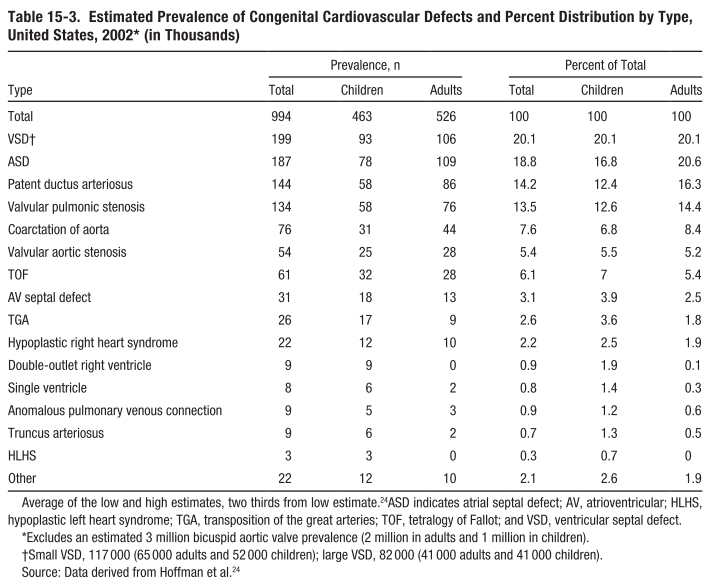
\includegraphics[width=0.6\textwidth]{2/chd-defects-usa.png}
\label{ch2:fig:usa-defects-prev}
\caption{Table of prevalences of congenital heart defects borrowed temporarily from \cite{Mozaffarian2016}.}
\end{figure}

% Diagnosis
The process of diagnosing CHD can begin before birth. A specialized ultrasound test called fetal echocardiography can detect heart abnormalities as early as the second trimester of the pregnancy. Additional tests, such as amniocentesis and follow-up ultrasounds may be needed to determine treatment options. Generally, severe CHD cases present and are detected at earlier stages, but minor defects may not become apparent until the patient is older. 
The incidence of CHD in live births vary across countries and continents: the United States reports approximately 4-10 CHD case per 1,000 live births, while Europe and Asia see about 6.9 and 9.3 CHD cases per 1,000 live births \cite{Mozaffarian2016}.
%It is important to note that these incidence rates only report the incidence of CHD as detected at birth, not cases detected later in the patient's life. % Is this correct?
A breakdown of prevalence rates of some of the most common lesion types can be seen in \ref{ch2:fig:usa-defects-prev}.
As screening tools become more effective, it is expected that these rates will increase as defects are detected earlier. % See (16)

Once a patient is diagnosed with one of these defects, the specific nature of his case must be clearly documented. The documentation of CHD using the International Classification of Diseases, Ninth Revision, Clinical Modification (ICD-9-CM) has 25 high level codes representing various presentations of CHD, but these codes used on their own are often not sufficient for describing a patient's true condition \cite{Mozaffarian2016}. Additional ICD-9-CM codes may be used to communicate the finer details of a patient's condition. 

%Depending on the cause of the 

Financial burden: high for certain defects, medium costs for surgical interventions for other lesions, still processing \cite{Mozaffarian2016}

% Complications and risks
Complications and comorbidities: heart failure, infections? Children with CHD at 19-fold risk for stroke (216) \cite{Mozaffarian2016}

Mortality: still processing information. Overall, the mortality for CHD patients is declining.  \cite{Mozaffarian2016}

% When are patients diagnosed?
% Expected lifespan
% Treatment plan
% Financial burden

\subsection{From Long-Term Risk of Hemorrhagic Stroke in Young Patients with CHD}
Giang et al performed a study comparing the prevalence of cardiac conditions in patients with and without CHD born between 1970 and 1993 in Sweden. They found that patients who had a CHD diagnosis were at about eight times higher risk for intracerebral hemorrhage and subarachnoid hemorrhage than their non-CHD counterparts. The CHD patients were also more likely to suffer from arrhythmia and heart failure.

\section{CHD AND NEURODEVELOPMENT}

Recent research has found that there is a link between CHD and neurodevelopment.

To address:
\begin{itemize}
\item Common combinations
\item Joint treatment?
\item Additional risks?
\item Joint financial and emotional burden on caretakers? 
\item CHD, neuro, and aging? Dementia/Alzheimer's?
\end{itemize}

\section{RESTING-STATE NETWORKS}

The idea of a neuronal network which operated when a person is at rest was proposed in 2001, and then confirmed in 2003 \cite{Raichle2001} \cite{Greicius2003}. Resting-state networks are recorded using resting-state functional magnetic resonance images (rs-fMRIs). rs-fMRIs are sequences of image volumes acquired over a period of a few minutes while the patient is in a task-free state. The image volumes themselves have relatively low spatial resolution when compared to structural MRIs, but their temporal resolution is significantly higher as a new volume is acquired every two to three seconds. Each volume records the blood oxygen level dependent (BOLD) signals within the brain at that point in time. 

The BOLD signals in rs-fMRI image sequences are analyzed using a process called functional connectivity analysis. Functional connectivity analysis identifies patterns and networks of brain activity. Because the patient is not performing a specific task during a rs-fMRI acquisition, these resting-state networks have the potential to reveal valuable information about a patient's neurodevelopmental status. Some functional connectivity analysis studies have lead to the discoveries of links between specific disruptions in these naturally occurring networks and neurodevelopmental diseases such as autism and attention deficit hyperactivity disorder \cite{Assaf2010} \cite{Zang2007}. With further refinements of both acquisition techniques and characterization of these functional networks, clinicians may be able to use rs-fMRI in early detection protocols to evaluate the neurodevelopmental status of infants and neonates, and in personalized care by identifying patients who may benefit from certain therapies or neuroprotective interventions.
